\documentclass[11pt]{article}
\usepackage{fullpage}
\usepackage{times}
\usepackage{graphicx}
\usepackage[round,sort]{natbib}
\usepackage{wrapfig}
\usepackage{caption}
\usepackage{boxedminipage}
\usepackage{url}
\usepackage{pdfpages}
\usepackage[compact]{titlesec}
\begin{document}

\renewcommand{\topfraction}{0.85}
\renewcommand{\textfraction}{0.1}
\renewcommand{\floatpagefraction}{0.75}

\newcommand{\note}[1]{\marginpar{\small{}\it{}#1}}

\newcommand{\ourtitle}[1]{\noindent\begin{tabular}{c}\begin{tabular}{l}\bf{}SHF: Small:
    Collaborative Research: Designing a Patient-Oriented Prescription
    Language:\\\bf{}An Executable Medical Algorithm for Gestational Diabetes Mellitus{}#1\end{tabular}\end{tabular}}


\newcommand{\poppl}{POP-PL}
\newcommand{\beginwfig}[1]{\begin{wrapfigure}{r}{#1}}
\def\endwfig{\end{wrapfigure}}

\pagestyle{empty}

\ourtitle{: Summary}

~

Preventable errors in healthcare are a leading cause of patient injury
and death~\citep{Kohn1999}.
%
Despite extensive effort and the expenditure of billions of dollars,
computerization has failed to solve this
problem~\citep{Landrigan2010}.
%
The PIs attribute this failure to a pervasive misunderstanding of the nature of
computation in healthcare.
%
While there has been a computer technology transfer in healthcare, we
await an intellectual transfer, in which software design,
maintainence, and debugging unlock the full potential of computer
science to improve healthcare.
%
The previous work of the PIs provides support for the claim that
\emph{a prescription is a program}, i.e., a medical algorithm.
%
This observation has the profound implication that knowledge
from computer science has direct application to the improvement of
healthcare performance.
%
This work has shown that software design and debugging of a
\emph{paper} prescription markedly decreases the rate of injury and
death associated with use of opioids in hospitalized patients
\citep{Belknap2008}.

There remains a knowledge gap: can we design a programming language
and adapt software engineering techniques to implement and maintain
highly reliable \emph{electronic} prescriptions?
%
To find out, the PIs will design and build the Patient-Oriented
Prescription Programming Language (\poppl{}) and evaluate if this new
platform can be used to improve management of the high blood sugar
levels that sometimes occur in pregnant women.
%
This condition is referred to as Gestational Diabetes Mellitus (GDM).


The need for prevention and treatment of Gestational Diabetes Mellitus
(GDM) in the US is projected to double to 600,000 women over the next
3 years due to increasing maternal obesity and a lower diagnostic
threshold.
%
Limitations of current GDM management include low patient adherence,
modest efficacy of interventions, time-burden for clinicians, and
cost.
%
The PIs will use \poppl{} to create POP-GDM, an e-prescription to be
initiated early in the pregnancy of women at increased risk of GDM.
%
POP-GDM will help the PIs continually monitor patients and clinical
processes, identify omitted or delayed tasks and remediate them,
detect conditions requiring action, notify patients and clinicians,
and facilitate corrective action.

\noindent
\textbf{Intellectual Merit.}  
%
The PIs expect this work to generate multiple new insights regarding the
building and maintenance of multi-stage programs, the development of
new kinds of analyses of programs, and the discovery of new general
methods for developing high-reliability software that facilitates
collaboration between machines and humans.
%
Computer science has long been driven by application areas; from the
early days of missile-targeting systems, to the development of
scientific computation, to creation of data-security solutions, core
computer science discoveries have often been made because of a need to
solve a particular problem.
%
Given the power of the tools we will use and the cross-disciplinary
expertise and experience of the team we have assembled, the proposed
work is a tractable challenge that will produce important new insights
in computer science.
%
Suboptimal healthcare represents a major burden on patients, leading
to worse patient outcomes and/or higher cost. 
%
The work in this proposal will eventually lead to reduction in
preventable adverse events, therapeutic failure, medical error, and
waste. 
%
Such solutions are urgently needed if our society is to apply medical
knowledge to the advancement of the health of patients.

\noindent
\textbf{Broader Impacts.} The GDM \poppl{} program will lead
to powerful tools for management of GDM in general obstetric practice
in the US.
%
More broadly, \poppl{} will give clinicians a public-domain,
open-source framework for designing, creating, debugging, and managing
a broad array of prescriptions for other medical problems; give
researchers tools for acquiring data about the effect of healthcare
interventions; and eventually provide a simple, inexpensive means for
conducting cohort studies, statistical process control trials, and
randomized controlled trials.
%
The work proposed here and along the anticipated future research
trajectory will favorably impact all who interact with the healthcare
system: patients, clinicians, and researchers.

\noindent
\textbf{Key Words:} programming languages; domain-specific languages; debugging; medicine; prescriptions

\newpage

\setlength{\parindent}{0pt}
\setlength{\parskip}{1ex plus 0.5ex minus 0.2ex}

\setcounter{page}{1}
\pagenumbering{arabic}
\pagestyle{plain}

\ourtitle{: Description}

~

\section{Introduction}

According to a report published by the Institute of Medicine of the
National Academies~\citep{preventing-medical-errors}, patient errors
are prevalent and a cause of serious concern.
%
The report points out that while there is wide variation, ``on average
a hospital patient is subject to at least one medication error per
day.''
%
A study of data from 1993 estimated that inpatient errors cost \$5,857
per patient~\citep{bates-et-al-1997}, leading the National Academies
report to extrapolate to a nationwide cost of \$2.3 billion annually
(in 1993 dollars).

Others have noticed this problem and have responded by trying to
introduce computers to the process of prescribing medicine to
patients, using systems collectively dubbed Computerized Prescriber
Order Entry (CPOE).
%
When carefully implemented, CPOE has been shown to reduce the rate of
medication prescription errors but clinically-relevant benefits, such
as improving clinical outcomes or preventing patient deaths or
injuries have not yet been clearly demonstrated~\citep{vanRosse2009}.
%
Even in terms of error prevention, CPOE's introduction to the hospital
has been a mixed blessing.
%
Certain medical errors, such as those related to poor handwriting, are
reduced but other familiar errors continue to occur and some new types
of error are introduced by CPOE.
%
In one report, CPOE actually \emph{caused} 22 types of medication
error; problems included fragmented display of drugs, inventory
display mistaken for dose guidelines, duplicate and incompatible
orders, and inflexible formats~\citep{Koppel2005}.

Prescribers routinely compensate for CPOE's awkwardness by supplementing the prescription data they enter in structured fields with free-text instructions and additional verbal instructions to nurses and pharmacists. We were the first to point out that prescriptions are programs and thus require a richer syntax than is provided by existing CPOE software.
%
A large study found 1\% of prescriptions had free-text instructions
inconsistent with structured data fields and 20\% of these
inconsistencies risked moderate or severe patient
injury~\citep{Singh2009}.


Compared with previous paper prescriptions, CPOE impairs
synchronization and feedback mechanisms in nurse-physician
collaborations~\citep{Pirnejad2008}.
%
Clinicians have difficulty understanding CPOE prescriptions because
they are presented as decontextualized fragments.
%
Paper provides a richer medium for prescribing than does a CPOE data
table display.
%
Intriguingly, others have recently begun applying
requirements gathering, software specification, and other software
engineering techniques to the construction of order sets
\citep{health-requirements-engineering}.


We expect that computerization will eventually dramatically improve the quality of healthcare. We attribute the failure of current healthcare computerization efforts to achieve meaningful gains to fundamental flaws in the conceptual basis of existing CPOE software. 
%
Put positively, we believe that:
%
\begin{center}
\textbf{a prescription is a program}
\end{center}
%
That is, a prescription requires ``a series of definite steps that
carry out a procedure'' or, in other words, an \emph{algorithm}.
%
The research areas of programming languages and software engineering
have amassed substantial knowledge about how to accurately implement an
algorithm as a program, and for dealing with the issues of clearly expressing and maintaining those programs. This knowledge is directly relevant to healthcare prescriptions.
%
In short, computers are not the missing piece to fix the problems of
medicine delivery, the \emph{intellectual contribution of computer
  science itself} is the missing piece.

Our approach, dubbed Patient-Oriented Prescription (POP), explicitly
acknowledges the algorithmic nature of prescriptions, leveraging the
power of programming to help clinicians model, test, debug, and
iteratively refine their patient management plans.
%
POP implies both algorithmic representation of prescriptions
\emph{and} application of a broad swath of software engineering
techniques, including modeling, testing, debugging, and interactive
refinement.
%
These techniques apply regardless of whether the prescription is
ultimately performed by computers or by people.
%
Indeed, our past work with patient-oriented prescriptions has
relied heavily on human performance of prescriptions.
%
CPOE systems are disconnected from clinicians' task lists,  resource availability data, and sequence or resource dependencies. It is common practice that clinicians obtain information from hospital CPOE systems and use this information to construct a separate task list. Attempts to integrate tasks, resource availability, and dependencies into CPOE have largely failed because CPOE software was constructed without an understanding of the algorithmic nature of prescriptions and medical orders. Effectively, CPOE is little more than electronic paper.
%
The next logical step is to bring to bear all the intellectual capital
inherent in algorithmic representation of prescriptions.
%
The fruits of this proposal will provide a means by which computers
and devices actively support clinicians in their efforts to provide
patients with safe, effective healthcare.

The remainder of this proposal explains how we've established the
foundation for prescriptions as programs and for supporting
domain-specific languages, how this has led to interesting research
questions in computer science, and how we expect to carry out a
significant effort to validate our approach at Northwestern University
Hospital.

\section{Background}

Our team includes members who bring a variety of complementary
technical strengths to address the opportunity presented by our
insight that prescriptions are programs. Belknap led a team who
implemented the first patient-oriented prescription, \emph{on
  paper}. Findler and Flatt built and maintain Racket, a platform for
building domain-specific languages. The next two subsections explain
our experience in more detail.

\subsection{Prescriptions as Programs}\label{sec:pap}

Physicians usually rely on memory and write extemporaneous
prescriptions. Occasionally, physicians use standard order sets or
templates~\citep{Elsberry1978,Honda1979,Kowalsky1982}, but these are
rarely derived explicitly from scientific
evidence~\citep{Fonarow2007,Dranitsaris2001}, often violate principles
of good software design, and are not verifiably debugged. Standard
order sets or templates have been shown to improve compliance with
drug therapy recommendations in some settings \citep{Girotti1990} but not in
others \citep{Aswapokee1992}. Prescription bugs in standard order sets can cause
catastrophic medication errors \citep{Cohen1992}.

The apparent simplicity of prescriptions is deceptive, as the
prescriber's terse instructions rely implicitly on subroutines:
toxicity and efficacy monitoring, pharmaceutical compounding, pharmacy
and nursing practices, operating instructions, laboratory methods, and
standard operating procedures. Neglect of scientific evidence, poor
design, and lack of adequate debugging of prescriptions and their
subroutines likely account for their erratic and occasionally fatal
effects. The recognition of the algorithmic nature of prescriptions
compels the application of software design principles and debugging
methods to their improvement.

The medical community has acknowledged that there has been no method
to ensure the rapid, reliable translation of detailed knowledge about
drug safety, efficacy, and cost into clinical practice. Clinical
practice guidelines have been variously criticized as being vague,
untested, non-rigorous~\citep{Weingarten1997},
obsolescent~\citep{Shekelle2001} and are largely ignored by
physicians~\citep{Cabana1999}. A recent, seminal study has found that
there has been little or no progress in improving the safety of
patients over the past ten years, despite advances in understanding
and mitigating some types of medical error~\citep{Landrigan2010}.

While it is possible for a physician to order drug therapy without
consulting relevant research articles, clinical practice guidelines,
expert opinions, textbooks, or lectures, a physician cannot order drug
therapy without a prescription. That is, the prescription is located
on the critical path between intent and practice. Well-formed, widely
used prescriptions exert beneficial effects through reduction of
clinical process variation, familiarity to clinicians, and
displacement of unsafe or ineffective practices. When properly
designed and debugged, prescriptions provide a conduit through which
evidence-based medical knowledge can reliably and safely reach patients.

We applied this insight to significantly reduce the risk of severe injury from medical use of opiods among hospitalized adults at St.\ Francis Medical
Center in Peoria, IL, a 731-bed tertiary care academic medical
center~\citep{Belknap2008}. During a 1 year base-line period, there were three to seven severe or fatal opioid-associated adverse drug events (ADEs) each month. After widespread adoption of POPA, the rate of severe/fatal opioid ADEs dropped to zero/month. Figure~\ref{fig:popa} shows POPA, the
complete program that we developed as part of our study.

Clinicians who use these patient-oriented prescriptions provide assiduous peer review, compelling the translation of new medical knowledge into improved
prescriptions. Sound prescription design followed by iterative cycles of hazard identification and debugging reduces the rate of severe patient injury by eliminating the prescription bugs that are a root cause of opioid-associated ADEs. POPA was subsequently implemented in two other hospitals. As POPA does not depend on resources that are unique to our hospital, we
expect that POPA is widely applicable.

Consider the subroutine for fentanyl dose reduction:
\begin{center}
\fbox{\scriptsize\begin{tabular}{ll}
\textit{Taper:} & 
\parbox[t]{5.2in}{STOP on-demand dose after (3 days) \underline{\hbox
  to 1in{}} (Alternatively, enter a stop date) \& \textit{then} REDUCE
continuous dose rate every 5 hours by (10) \underline{\hbox to .4in{}}
micrograms}\\
\end{tabular}}
\end{center}

\noindent
This fragment represents a subroutine that is executed by humans. This
human-oriented programming language 
includes conditionals, an optionally specified
variable with default value, an external (human) processor call, and
elements driving reconciliation with other subroutines. The phrasing
also employs TALLMAN lettering to emphasize the direction of
change. The content of this prescription is
evidence-based. Its structure was based on software design principles
and then debugged, through trial and error, deriving a form that is
clear to clinicians and accurate in performance. For example, 
constructions like TALLMAN lettering improved execution accuracy compared with
less redundant code. Unlike CPOE data tables
that obscure the hierarchical and modular structure of prescriptions,
this fragment of a \poppl{} program clarifies it, opening the door to 
the use of computer science techniques for improving the quality of
the program.

\begin{figure}
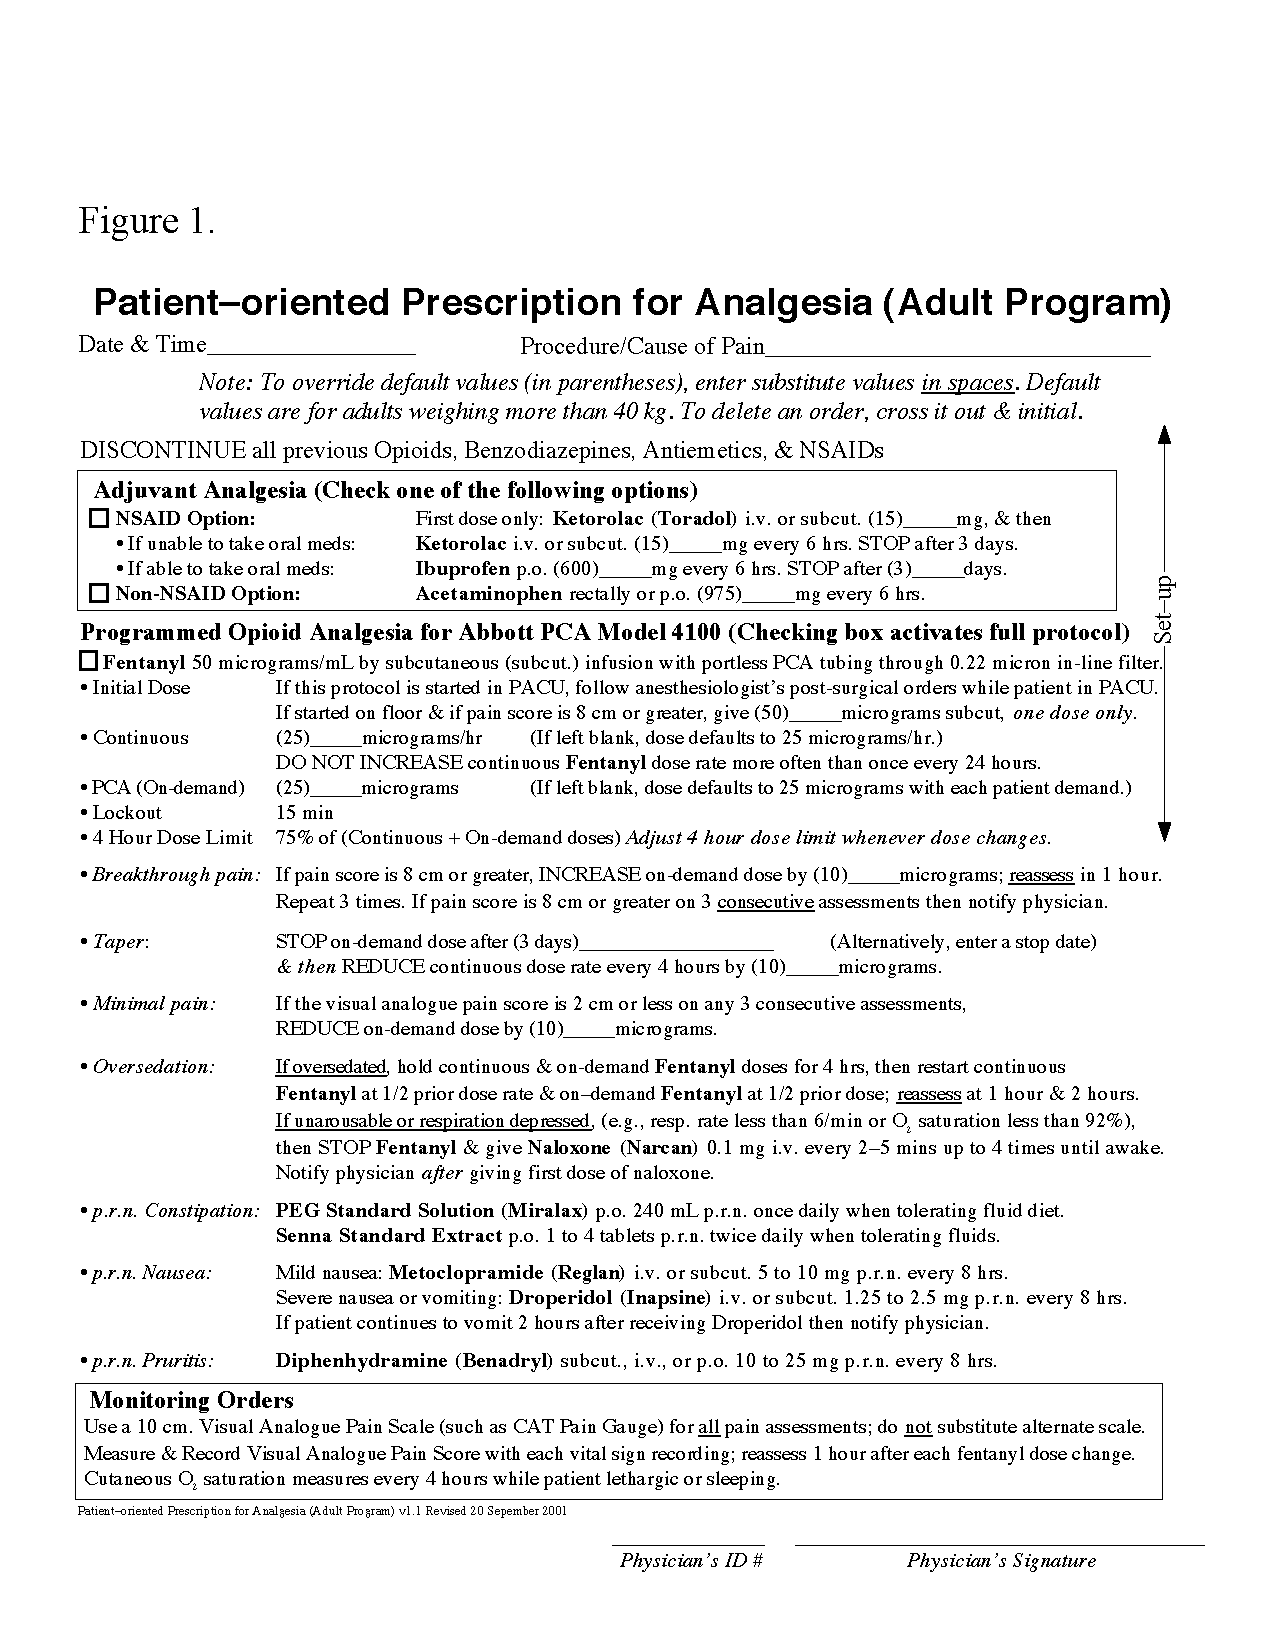
\includegraphics[scale=.8]{fig1.pdf}
\captionsetup{labelformat=empty}
\caption{}\label{fig:popa}
\end{figure}

 
To validate the success of our original \poppl{} program, we also
conducted a statistical process control clinical trial and nested
subcohort analysis in a population of 153,260 hospitalized adults. In
the orthopedics subcohort, POPA increased recording of pain scores
(94\% vs.\ 72\%, P $<$ 0.00001) and use of adjuvant analgesics (95\%
vs.\ 40\%, P $<$ 0.00001) and resulted in fewer opioid-associated
severe adverse drug events than routine patient-controlled analgesia
(PCA) (0\% vs.\ 2.7\%, number needed to treat (NNT) = 35, P $<$
0.015). Hospital-wide, POPA use increased to 62\% of opioid
prescriptions (diffusion half-life = 98 days), while opioid-associated
severe/fatal adverse drug events fell from an initial peak of seven
per month to zero per month during the final 6 months (P $<$ 0.0016)
of the study, as shown in Figure~\ref{fig:popa-results}.

\begin{figure}
\begin{center}
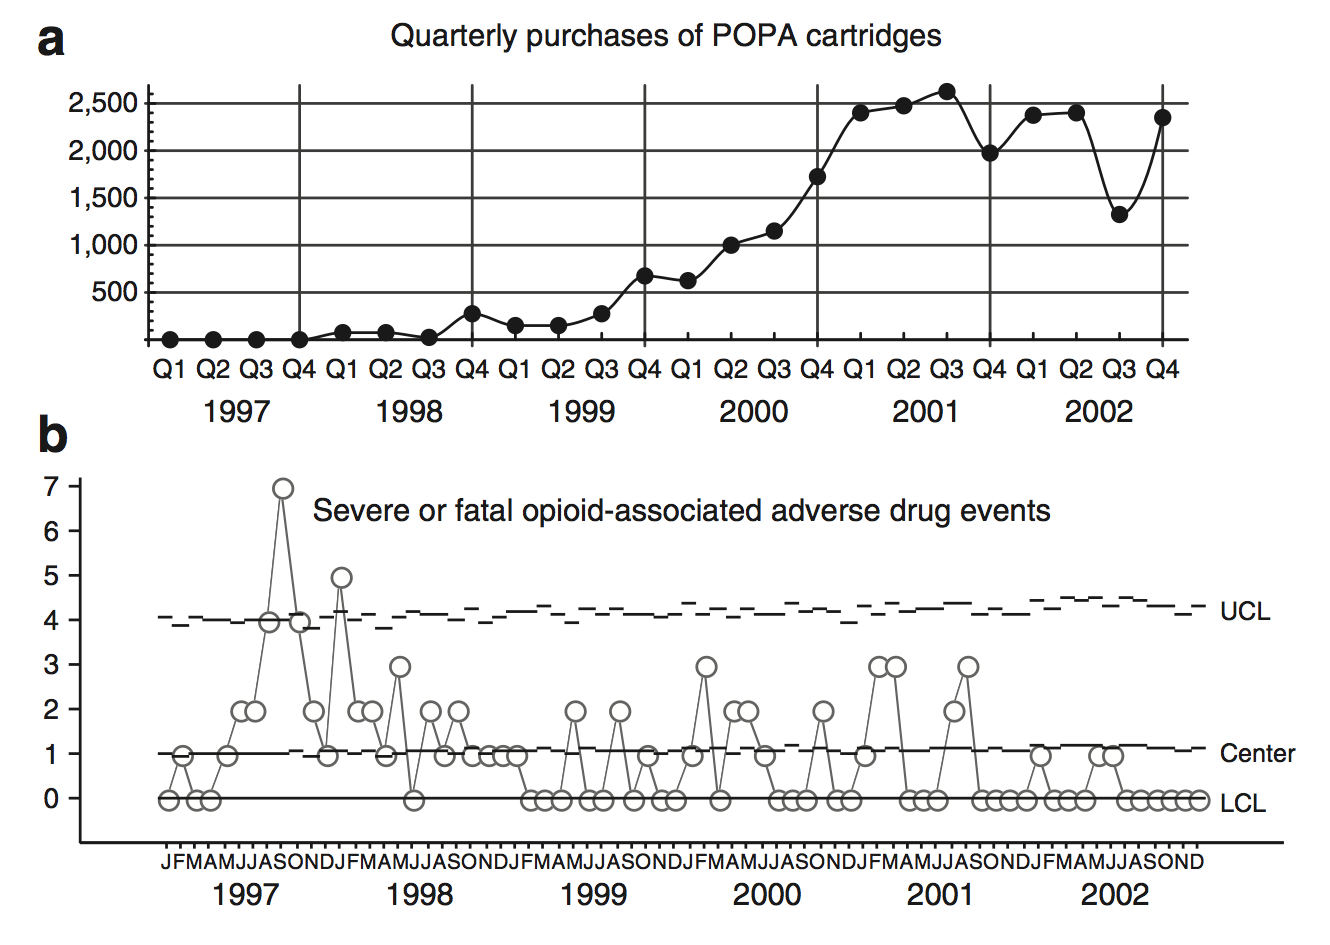
\includegraphics[scale=.2]{popa.png}
\end{center}
\caption{POPA Trial results}\label{fig:popa-results}
\end{figure}

The success of the POPA was due in part to the rigor that algorithmic
thinking brought to the process of building the prescription and in
part to extensive debugging. This proposal aims to build, test, and
deploy the software required to make \poppl{} programs
machine-executable, interoperable with other healthcare software, and
available for clinical trials in routine clinical environments.

\subsection{Specialized Programming Languages in Racket}\label{sec:racket}

The Racket programming language~\citep{Racket} offers an extensible
core language, and the DrRacket programming
environment~\citep{DrSchemeJFP} is (by design) adaptable to language
extensions. The environment part of the equation is crucial, because
domain experts need more than a compiler and run-time system to
develop programs. They also need a full suite of development tools,
including program editors, interactive evaluators, debuggers,
syntax-coloring editors, and documentation tools. Prescribers write
complex medical algorithms and are familiar with algorithmic thinking
but very few have any formal knowledge of programming. Thus, a key
design element for POP-PL will be usability by prescribers with little
formal knowledge of computer programming. There are numerous instances
where such software has been constructed in other domains; consider,
for example, that administrative assistants use Excel and machine
operator at Caterpillar Tractor program lathes. These are domain
specific languages that allow people to program with little formal
training. Doctors are programmers too; they write prescriptions and use
order sets~\cite{Elsberry1978,Honda1979,Kowalsky1982}. These are
rarely derived from evidence~\cite{Dranitsaris2001,Fonarow2007}, often
violate software design principles, and are not verifiably
debugged. Standard order sets increase use of best practices in some
settings~\cite{Girotti1990} but not others~\cite{Aswapokee1992}. Bugs in order
sets can cause catastrophic errors~\cite{Cohen1992}.

VisiCalc, the first spreadsheet app, resembled paper accounting
worksheets but revolutionized accounting and finance because it did
something radically different, auto–calculating data cell values
according to formulas programmed by the user. Previously, this work
required calculators, pencils, and paper, and was laborious and
error-prone. Our task here is similar; the design and implementation
of POP-PL, a prescribing language, will be a process of discovery, as
we study the (often elegant) prescriptions clinicians already use. We
expect to develop a language that will leverage the existing
knowledge, tropes, and structures that physicians and other
prescribers have. We envision an ``active prescription'' that
superficially resembles a paper prescription in the same way that the
GUI of Excel resembles a paper spreadsheet.

DrRacket is best known in its role as a tool for
teaching; the teaching dialect of Racket is not the full language, but a series of
languages designed for progressively more advanced
students---domain-specific languages for introductory programming.
Other domain-specific languages that are embedded in
Racket include the Redex language for developing and testing
operational semantics~\citep{Redex}, the web-server framework for
transparently implementing web services via sessions managed over
HTTP~\citep{web-server,mccarthy09,mccarthy10}, the Slideshow language
for creating slide presentations~\citep{Slideshow}, the Scribble
language for documentation and typesetting other forms of prose~\citep{Scribble}, and
the Margave tool for security policy verification~\citep{Margave}.

Of these, Margave most closely resembles the use of Racket  we have in mind
for prescription programs. Experts in the domain of security protocols
use Margave as a language within DrRacket, but do not write
Racket code at all. Instead, they treat DrRacket as a kind of
``DrMargave,'' since writing a module in the Margave language causes 
DrRacket to adapt to that specific domain language.

Racket's underlying language-definition technology is based on
Lisp-style macros---specifically, the lexical-context preserving macro technology that evolved in
Scheme~\citep{R6RS}. Racket builds on this foundation with a 
richer API for macro transformers to manipulate and inspect syntactic
terms. This API is powerful enough, for example, to implement the
continuation-passing transformation of the web-server
framework~\citep{mccarthy09}, the type checker for a
statically typed dialect of Racket~\citep{TypedRacket}, as well as the
Racket class system itself \citep{fff:scheme-classes-mixins-traits}. Macros are
integrated into a module layer that enables different languages and
language extensions to compose within a larger program.


\section{Proposed Work}

\addtocounter{subsection}{-1}
\subsection{Understanding Best Practices}\label{sec:best-practices}

To begin, we will conduct an exhaustive search of the medical
literature, interviews of domain experts, clinical practice
guidelines, and many examples of prescriptions/protocols/institutional
practice guidelines so as to identify very fine-grained descriptions
of the ``medical algorithms'' used to manage GDM.

\paragraph{Expected outcomes.}
From this comprehensive survey, we expect to gain a better
understanding of the variety of approaches that clinicians use to
manage GDM. This survey process was previously developed by us for the
purpose of developing patient-oriented prescriptions for other medical
problems.  We expect this survey to serve as a crucial source of ideas
and insights as to how one might implement a successful \poppl{}
program for managing GDM and also to better understand how \poppl{}
programs will work in general.

\subsection{Event-based Programming}\label{sec:new-start}\label{sec:event}

From past work on POPA, we expect that the large-grain structure of a
\poppl{} program will describe how to react to various kinds of
events, in a general sense.  For example, consider another fragment of
the POPA program in figure~\ref{fig:popa}:
\begin{center}
\fbox{\scriptsize\begin{tabular}{ll}
\textit{Breakthrough pain:} &
\parbox[t]{5in}{If pain score is 8 cm or greater, INCREASE on-demand dose
  by (10) \underline{\hbox to .3in{}} micrograms; \underline{reassess} in 1 hour. Repeat 3 times. If pain
  score is 8 cm or greater on 3 \underline{consecutive} assessments then notify
  physician. } \\
\textit{Minimal pain:} &
\parbox[t]{5in}{If the visual analogue pain score is 2 cm or less on any 3 consecutive assessments,
REDUCE on-demand dose by (10) \underline{\hbox to .3in{}} micrograms.}
\end{tabular}}
\end{center}

This fragment covers two responses to a patient's pain scores; the
first covers the situation where the patient has increased pain and
the second when the pain decreases. In each case, the instructions are
guarded by a condition that spans some unspecified time.

\poppl{} programs consist of a series of interconnected fragments
based on real-world events, e.g., the patient indicating pain
severity, or a nurse noticing that a patient is unconsciousness, or
that a pulse oximeter detects that a patient's capillary blood O$_2$
saturation has fallen to a low level.

We expect to build on ideas from function reactive programming
languages~\cite{frp} and guarded commands~\cite{guarded-commands}.
Adapting these techniques to our setting poses interesting challenges,
however. In particular, tasks can compete for resources including
clinician time with other tasks in other prescriptions, and may
require human judgment, decision-making, and validation. For example,
POPA (Figure 1) begins by \emph{discontinuing} previously prescribed
drugs with potential for dangerous interactions with fentanyl, the
opioid used in POPA. In our vision of how these ``prescription
collisions'' will be handled in \poppl{} programs, each prescription
will specify a process to follow so as to resolve such collisions
instead of having a simple priority based approach with automatic
resolution.

A prescription is more like a reactive system in the domain of
embedded systems for controlling cars or airplanes. When an airplane's
engines fail, the response includes output of software on the
airplane, software on other airplanes, software in the control tower,
and humans in each of these settings.  The interactions are complex
and the stakes are high. Car and airplane software domains currently
require programmers with high expertise who usually work at a low
level. Fortunately, the time scale for executing a prescription is
orders of magnitude higher, and the available computing resources are
orders of magnitude greater. We will be able to concentrate more on
designing a simple and expressive language and less about how to map
the programming model to constrained devices. 

\paragraph{Research questions.}
What is the language that \poppl{} programmers should use to describe
events and event–patterns? How can we, given a \poppl{} program,
determine if all of the possible events are covered and there are no
redundant patterns? Lack of coverage could mean that important
information is being dropped (e.g., a patient's requests are being
ignored) and redundancy could mean that conflicting responses could
come from a particular stimulus.

\paragraph{Expected outcomes.}
We expect to develop new languages for describing event streams and
patterns of event streams, influenced by the way medical practitioners
and patients and devices respond to each other. In addition, we expect
to build new analyses that determine if a set of event patterns cover
all possible sequences of events and if a set of event patterns are
redundant.

\subsection{Iterative Refinement \& Debugging}\label{sec:iterative}

Iterative refinement~\citep{boehm:spiral} is crucial for any program
at the complexity of patient-oriented prescriptions and \poppl{})
programs. For example, in the initial version of the POPA program,
there was no Ibuprofen option (only Ketorolac and Acetaminophen
options). After some testing, it was discovered that Ibuprofen was
also needed and this initiated a refinement to the program. The team
collaboratively revised POPA over several iterations, then tested the
new prescription in simulation over several more iterations. Then, a
pilot study in a limited number of patients was conducted, after which
the change was released and used with all patients. After deployment,
statistical sampling and analysis was used to assure that the improved
version of POPA did not inadvertently introduce new problems in
routine practice.

Of course, iterative refinement is a standard part of software
engineering lore. What is different for \poppl{} programs is the
nature of the iterations---some parts require people to simulate
them. We expect that computational power can be used to increase the
efficiency and productivity of the \poppl{} software developer and of
the clinicians who perform the prescription.  Once prescriptions are
in a machine-executable form and input events are collected into a
machine-processable form, then variations on programs can be run on
the same inputs to check that a new version works as expected. That
is, the developer of a prescription needs a regression test suite and
new test cases to check new versions of the prescription.

\paragraph{Feasibility} 
Physicians and other prescribers do not have formal training in
computer programming but do have extensive experience writing actual
prescriptions. This prescription-writing experience is effectively a
parallel discipline that uses many constructs common to computer
programming but without the benefit of the extensive conceptual
framework provided by computer science.  Thus, our task is not to
create this language de novo but instead to create an intuitive
language for these prescribers that will be formally defined and more
robust, reliable, and powerful than free text.  To improve the
feasibility of iterative refinement, we plan to build a replay
mechanism into \poppl{} so that the stream of events from one run of a
program (including all of the actions taken by the patients and the
care-givers) can be used to simulate how a new \poppl{} program
runs. In the previous paper versions of POPs, manual review of medical
records and direct observation of the clinical process by humans was
used to gather information for purposes of debugging. Much of this
data–gathering can be automated for e-prescriptions, as the POP-SE
environment will capture a rich data-stream of clinical events.

\paragraph{Research questions.} How can we determine if the replay of
a \poppl{} program has failed because there is a bug in the program or
because some intended change to the program has invalidated the trace?

\paragraph{Expected outcomes.} We expect to define a notion of
well-formed trace and a compatibility notion between traces and
programs. Specifically, a well-formed trace will be compatible with a
\poppl{} program if and only if an error that results from running the
trace is due to a bug in the program.

\subsection{Staged Programming}\label{sec:staged-programming}

One of the most exciting directions for integrating computing into
medicine is in moving off of the desktop. Any given \poppl{} program
executes on a variety of machines and contains instructions for both
machines and humans. Consider, for example, this fragment of a
\poppl{} program that deals with one part of the daily glucose
monitoring of a GDM patient:

\begin{center}
\fbox{\scriptsize\begin{tabular}{l@{~~$\bullet$~}l}
\textit{Initial diagnosis:} &
\parbox[t]{5in}{Advance practice nurse tells the patient to measure
  the blood glucose level every morning between 5 and 8am.} \\
\textit{Daily monitoring:} &
\parbox[t]{5in}{Alert patient if no glucose level value received by 8:30} \\
&
\parbox[t]{5in}{Alert nurse if no glucose level value received on
  three subsequent days.}\\
&
\parbox[t]{5in}{If glucose value between 120 \& 140, patient to adjust
dose}\\
&
\parbox[t]{5in}{If value higher, consult advance practice nurse}\\
\end{tabular}}
\end{center}

This code fragment has machines talking to machines (the glucose meter
communicating with the cell phone, pager, or telephone of the patient
as well as communicating with the hospital to relay the data values),
machines talking to people (e.g., alerting the patient when no value
has been received), and people talking to people (the nurse informing
the patient of those parts of the prescription dependent on the
patient). This fragment is only a small fragment of the program.

In the same way that a playwright works on a single play and
distributes the ``work'' of the play to different actors, the
developer of a prescription wants to develop a single program rather
than separate programs for all of the different actors in its
execution. Precedents for splitting a single program into multiple
roles exist in the computing domain, including the problem of
splitting a web-based application into server-side and client-side
parts, which we have investigated previously~\citep{mfgkf:asej2004}.

In general, the problem is difficult, but usually because the problem
is splitting a traditional linear program into a concurrent system.
We expect \poppl{} programs to use an event-driven style that is
inherently concurrent and that more easily translates into real
devices and human actors. The problem is not as easy as extracting the
subset of a play that contains a single actor's lines, because events
will trigger cooperative responses from many different actors, but the
problem is still far easier than extracting concurrency from a
traditional single-threaded computation.

Additionally, \poppl{} programs can provide functionality that would
be highly desirable to clinicians. For example, clinicians must
simultaneously care for large numbers of different
patients. Interruptions are frequent. Setting priorities is
challenging. Mapping the urgency and importance of each task tasks
onto a Cartesian grid would give us the ability to provide a more
informative visualization of the available tasks, and thus permit
clinicians and patients to make more informed decisions. We expect
that providing this functionality would improve the effectiveness of
clinicians and would also diminish the stress inherent to a demanding
clinical environment.

\paragraph{Research questions.} How can we write \poppl{} programs so
that the roles of the various players (machines and people) are
separable? Can we automatically generate internally consistent views
of a \poppl{} program that are specialized for particular people and
understandable by those people? Similarly, can we automatically
generate internally consistent programs that run on the myriad of
devices given just a single \poppl{} program?

\paragraph{Expected outcomes.} 
We expect to build on ideas of staged
programming~\citep{multistageprogramming,
  efficient-program-specialization, runtime-generation-c,
  tickc:toplas} and aspect-oriented programming~\citep{aop} to come up
with a notion of staging that captures these very different parts of
\poppl{} program.

\subsection{Virtual Machines and Medical Devices}\label{sec:new-end}\label{sec:vm}

Following up on the problem of splitting a \poppl{} program into 
different pieces for different devices, we will need a platform
for actually running the pieces on the different devices and having
the devices communicate with each other successfully. We will design a
relatively high-level virtual machine language that is easily
retargetable to multiple different low-level, programmable devices.

Intermediate languages like the JVM~\citep{jvm} and the CLR~\citep{clr}
already provide guidance and even tool support for running on many
different programs, but few medical devices currently support running
such general purpose programs. We plan to develop a simple, highly–intuitive,
restricted language that is better suited to environments where
information must be carefully protected and to implement this language on various medical devices.

Our approach includes four steps 1) A threat and risk assessment
documenting the system components, the stakeholders, the security
requirements, and the threats against those requirements, 2)
Operational security guidelines describing countermeasures, technical
or otherwise, that mitigate security threats, 3) A policy document
describing goals, responsibilities, guidelines, and procedures, and
finally 4) A security architecture that accurately reflects the
security priorities and priorities for the prototype framework.  This
architecture will act to place \poppl{} in a secure sandbox isolating
the language from interactions with hardware devices and EMRs.

\paragraph{Research questions.} How can we restrict the computational
power of programs in our intermediate language to ensure that
information only goes to trusted recipients? 

\paragraph{Expected outcomes.} A new low-level language for medical
devices that guarantees security properties.

\subsection{Workflow Management Systems}

Workflow management systems are computer systems that monitor and
manage tasks performed by humans (and computers). These systems accept
the specification of some set of tasks and their dependencies and
outcomes and then accept input from humans to ensure that the proper
set of tasks occur in the proper order.

Most of these systems are too brittle for our needs, as they are not
generally programming languages, but instead GUI-based applications
that only allow partial specification of the tasks and their
dependencies, as such specifications quickly become too complex for
that kind of setting.

One notable exception is iTasks~\citep{itasks}. It is a
domain-specific language embedded in the programming language Clean
for the specification of tasks and their interactions. iTasks allows
programmers to specify workflows in a high-level, declarative manner
whereby tasks are composed out of atomic tasks and combinators that
express sequential composition or parallel composition (for
example). It also has excellent support for automatically building
GUIs for data entry based on type specifications. We expect to build
on the ideas in iTasks and specialize them to the medical setting.

\paragraph{Research questions.} One challenge in the medical
setting is that a specific task can change over time. For example, a
naive understanding of the directive ``take medication every 6
hours'' would lead to an inflexible timer that expects a patient to
either check a box or not at the pre-determined times. However, many different tasks compete for completion and many events potentially alter the precise timing of prescribed actions; further,
there is a notion of time built into that specification; taking the drug
dose 20 minutes early or late is probably fine (depending on the
medication and dosage guidelines), but if two hours have elapsed
since the correct time, then waiting for the next interval is
certainly the wrong behavior. Instead, the proper course might be to adjust the future drug dose schedule to catch up. The details of what these dose and schedule adjustments ought to be are often quite clear to the prescriber or pharmacist but are almost impossible to express clearly within the constraints of existing CPOE systems. So we need to understand how to include a notion of time into POP-PL prescribing models that allow a task to gracefully change over time.

We expect the core model of a prescription to be event-driven and we expect to apply the considerable expressive power of Racket to build prescription language constructs that intuitively and robustly express how medical tasks can be accomplished within an event-driven model.

\paragraph{Expected outcomes.} A notion of interoperability for
combining iTasks-like specifications with event-driven programming,
and a way to introduce a notion of time into iTasks.


\section{Experimental Validation}

Our plan to evaluate the design of \poppl{} is to develop a program
(which we call POP-GDM) for the care and treatment of gestational
diabetes mellitus (GDM), and to conduct a simulation of a clinical
trial at Northwestern Memorial Hospital.

\subsection{GDM Background}

Due to rising maternal obesity and lower diagnostic threshold, GDM cases
will double to 600,000 women over the next 3 years. A crisis looms, as
resources are inadequate to manage this projected patient load. GDM
raises risk of stillbirth, C-section, and
pre-eclampsia~\citep{Langer2006} and has long-term effects, including
raised risk of impaired glucose tolerance in adult
offspring~\cite{Metzger2007}. The Hyperglycemia and Adverse Pregnancy
Outcome (HAPO) study of 25,000 pregnant women showed that adverse
outcomes in mother, fetus, and neonate rise with maternal glycemia at
24--28 weeks~\cite{Metzger2008}. A Swedish study found 20\% of
pregnant women at risk for GDM and a surprisingly low rate of GDM
screening~\cite{Persson2009}. Given similar trends in the US, an
opportunity remains for improvement of pregnancy outcomes through
higher efficacy interventions.

GDM treatment lowers perinatal morbidity and improves maternal quality
of life~\cite{Crowther2005}. There is a 2- to 4-fold increase in
metabolic complications and macrosomia with untreated GDM; treatment
eliminates this gap~\cite{Langer2005}. One of us was a PI for a
multi-center randomized control trial in women with mild GDM in the
24th--31st week of gestation~\cite{LandonPeaceman2009}. In this study in
958 women with abnormal glucose tolerance but fasting glucose $<$ 95
mg/dL, treatment reduced birth weight (3302 vs. 3408 g), neonatal fat
mass (427 vs. 464 g), birth weight $>$ 4000 g (5.9\% vs. 14.3\%),
shoulder dystocia (1.5\% vs. 4.0\%), Cesarean section (26.9\%
vs. 33.8\%), and combined gestational hypertension + preeclampsia
(8.6\% vs. 13.6\%; P=0.01). Based on these encouraging results and the
significant residuum of hyperglycemia seen in the treated cohort in
these clinical trails, we expect our POP-GDM program, with better
performance, will further improve outcomes.

\subsection{Simulation Facility Background}

A particular strength of this application is access to the unique,
separately funded, Medical Simulation and Immersive Learning Center
at the downtown Chicago campus of
Northwestern University. It provides simulation environments including
physical plant, electronic devices, and computers of (1) a 5-bed ICU,
(2) an ambulatory clinic, (3) a work area for interacting by phone,
text-messaging or email with patients at home, and (4) equipment and
support for producing high quality video for use in mastery learning
modules we will develop for clinicians and patients. We will use this
facility to conduct simulation trials of POP-GDM in successive cycles
of refinement and debugging. 

\subsection{Simulation Trial for POP-GDM}

Our simulation trials for POP-GDM will not involve real patients and
thus will not have the possibility of harming people.  That lack
aside, our simulation trials will be as realistic as possible. 

In particular, we plan to collect data from real patients, including
their diet, glucose readings, and (if necessary) insulin intake. 
%
We expect this data to be available in significant quantities as we
expect there to be 300 women with GDM to be seen in the Maternal-Fetal
Medicine Clinic at Northwestern Prentice over the 2 year enrollment
period for this proposal. 
%
We plan to use this data to perform pure computer-based simulations
that will help us determine how our POP-GDM program will respond to
real-world data.

We also plan to perform simulations with real clinicians, actor
patients, and simulated inputs from glucometers and accelerometers
based on the data collected from the patients.
%
We will assess timeliness as the duration between reception by the
clinician of a message from a device, a patient, or another clinician
and complete transmission of a response by the clinician to the
patient.
%
We will assess appropriateness according to concordance
between the action initiated by the clinician and what is called for
by the consensus guideline established by our expert panel. 
%
We will assess reliability according to latency and consistency. 

The directory of the Northwestern Simulation and Immersive Learning
facility and will provide assistance and oversight for these
simulation trials.

\subsection{Evaluation}

We hope to validate that POP-GDM improves adherence to prescribed
diet and activity in women at high risk for GDM. Depending on the
strength of the therapeutic effect, we may also show that POP-GDM is
superior to usual care for improving maternal glycemia and for
reducing macrosomia, and for avoiding insulin. 


\section{Budget, Personnel, and a Cultural Chasm}

One difficulty we have struggled with in trying to find funding for
this project is the chasm that separates computer science and medical
culture.
%
In this proposal, this chasm is most evident in the budget. 
%
Our experience writing and reading SHF proposals has been that the
bulk of a conventional SHF budget goes to graduate student support,
followed by a month or so of salary for a PI, with travel,
equipment, and supplies making up a distant third.
%
This apportioning of funds fits will with the way most computer
science departments are organized, specifically with graduate students
that are in a position to make a strong contribution to the research
and faculty members who generally receive 9 months of salary
guaranteed by the university.
%
In contrast, even tenured biomedical faculty typically receive only
10\% of their salary guaranteed by the university.

Accordingly, our proposal includes four months of salary support for
Belknap, as compared with only one half of a month each for Findler
and Flatt.
%
Importantly, the difference in these numbers does not reflect a
difference in the level of commitment to the project from the PIs.
%
All three of us are equally and highly committed to improving the
state of the art in programming languages and software engineering by
bettering the practice of medicine and specifically prescriptions.


Simulation trials are expensive, and that expense is reflected in our
budget by the number of people involved.
%
Despite the expense, we believe that conducting a simulation is
critical to the success of \poppl{}.
%
That is, if we are to succeed in exploiting our motto that
prescriptions are programs, we must have the feedback from evaluating
or prescription programs in a true clinical setting.

The remainder of this section introduces the people we plan to be
involved in this project and what roles they play.

\begin{itemize}
\item\textbf{Robby Findler}; Findler is a Ph.D. in computer science;
  his dissertation improved the state of the art of software
  specifications, specifically how to state and enforce behavioral
  software contracts in a higher-order setting. He is one of the core
  members of the Racket development team and has helped to design and
  build many of the domain-specific languages discussed in
  section~\ref{sec:racket} of the proposal. Findler will be leading
  the development of the domain-specific language, focusing on the
  requirements gathering and language design issues, together with a
  PhD student.

\item\textbf{Steven Belknap}; Belknap is an M.D. specializing in
  Internal Medicine and Clinical Pharmacology. Belknap has extensive
  experience providing medical care hospitalized adults.  He also has
  training and experience as a computer programmer. His long–standing
  research interest has been ``algorithmic medicine''.  He is the
  first to have successfully applied software engineering and
  debugging methods to prescriptions for management of asthma,
  aminoglycoside antibiotic treatment of infections, anticoagulation
  therapy, and severe pain. Dr.\ Belknap was the principal
  investigator of a study involving more than 50,000 hospitalized
  adult patients treated with opioid analgesics as discussed in
  section~\ref{sec:pap}. Belknap introduced the main idea in this
  proposal, namely that ``A Prescription is a Program''. Belknap
  provides the overall vision and leads the clinical part of this
  project.

\item\textbf{Matthew Flatt}; Flatt is a Ph.D. in computer science; his
  dissertation improved the state of the art in modularity constructs
  for programming languages, specifically he designed, build, and
  proved properties of a new technique for mutually referential module
  systems. He is also one of the core members of the Racket
  development team and has helped to design an build many of the
  domain-specific languages discussed in section~\ref{sec:racket} of
  the proposal. Flatt will be leading the development of the runtime
  system to support \poppl{}, focusing on the back-end and
  infrastructure support at the Racket level. Flatt is the only team
  member not located in Chicago, but he and Findler have been
  collaborating over a long distance for a decade and he plans to make
  multiple trips to Chicago as part of this project.

\item\textbf{Dennis West}; West is a Professor of Dermatology and
  Pediatrics, a pharmacist, and Director of the Dermatopharmacology
  Program in the Department of Dermatology at Northwestern University,
  one of the largest such clinical research programs in the U.S. He is
  also Chair for Administrative Review with the Institutional Review
  Board for the Office for the Protection of Research Subjects at
  Northwestern University.  He served as Chair for the Dermatology
  Expert Panel at the United States Pharmacopeia from 2005--2010. West
  also leads RADAR (Research on Adverse Drug Events And Reporting), a
  proactive pharmacovigilance collaboration based at Northwestern, and
  has worked closely with Dr.\ Belknap for several years within RADAR
  and other pharmacovigilance projects. His role on this project will
  involve coordination with Walgreens and with the Pharmacy Department
  at Northwestern Memorial Hospital, and analysis and dissemination of
  results, with particular focus on the prescription design of the
  project.

\item\textbf{Boyd Metzger} Metzger is a physician specializing in
  Internal Medicine and Endocrinology. He has had a career-long
  interest in the perinatal and long-term consequences of GDM, the
  detection and diagnosis of GDM and its treatment. Metzger is a
  leading authority in the field of GDM. He led the seminal HAPO
  study~\citep{hapo}, which helped demonstrate the need for a lower
  threshold for intervention in GDM. He will provide domain expertise
  and advice in the area of GDM.

\item\textbf{Charlotte Niznik}; Niznik is an RN, Advance Practice
  Nurse and is the Maternal Fetal Medicine Specialist who coordinates
  the GDM program and the Maternal Obesity program at
  Northwestern. She has collaborated in preparation of this grant
  application and is a key source of insight and experience regarding
  the management of GDM.

\item\textbf{Alan Peaceman}; Peaceman is the Chief of the Division of
  Maternal/Fetal Medicine at Northwestern University Feinberg School
  of Medicine.  He currently serves as Principal Investigator for the
  National Institute of Child Health and Human Development (NICHD)
  Maternal-Fetal Medicine Units Network Grant. Peaceman will
  collaborate on creation of POP–GDM and will provide domain expertise
  and clinical advice regarding management of GDM.

\item\textbf{Bonnie Spring}; Spring is a Ph.D. clinical health
  psychologist. Her research aims to understand the biobehavioral
  mechanisms that maintain unhealthy behaviors and to develop and test
  interventions that promote healthy behavior change. She has many
  years of NIH- and VA-funded clinical trials experience intervening
  to promote healthy behavior changes in diet, physical activity, and
  smoking, singly or conjointly. Spring sees the proposed research as
  an important next step in understanding how to optimize multiple
  risk behavior change.

\item\textbf{John Vozenilek}; Vozenilek is an Emergency Medicine
  Physician and is the Director of Simulation Technology and Immersive
  Learning for the Feinberg School of Medicine. In this capacity, he
  provides central coordination and oversight for undergraduate,
  graduate, interdisciplinary, and continuing medical education
  programs. For this project, Vozenilek will provide advice and
  direction regarding the performance of the prescription simulation
  portions of this proposed work. He will also participate in data
  analysis and preparation of manuscripts.

\item\textbf{Susan Eller}; Eller is a nurse and is the Director of
  Interprofessional Education at Northwestern University Feinberg
  School of Medicine. She will provide oversight and assistance
  regarding the performance of the prescription simulations.

\end{itemize}

\section{Curriculum Development Activities}

Findler and Flatt have a well-established track-record of
curriculum-related community outreach, stemming from the
\textit{TeachScheme!} project and it's successor, \textit{Program by
  Design}. Both of these are centered around the text book \textit{How
  to Design Programs}~\citep{fffk:how-to-design-programs}.  This text
teaches the fundamentals of programming using a metodology structured
around design principles instead of more conventional approaches that
tend to be structured around the syntactic features in the programming
language being studied.

Although our curriculum development plans with regards to this
proposal are modest, we plan to leverage this experience to reach out
to medical professionals that are interested in programming to teach
them how to program in \poppl{}.

\section{Results from Prior NSF Support}\label{sec:prior-results}

\paragraph{Joint}

Flatt (University of Utah) and Findler have received one join NSF
research grant (CCR-03-06270: \textit{Collaborative: Exploiting Component Contracts for Static Analysis and Testing}, 2003--2005, \$270,947)

Along with their PLT colleagues, they wrote two invited papers in
Dr.~Dobb's Journal. These two papers discuss how to create little
languages with Racket's macro system and how to (almost)
automatically extend DrRacket, the programming environment, so that it
can cope with these embedded little languages. The projects have also
helped support development of Racket.

\paragraph{Findler}

Findler is a Co-PI on one current grant (CCF 1116610 \textit{SHF:
  Small: Integrating Compiler and Architecture Design to Boost Timing
  Speculation}, 9/2011--9/2014, \$493,399).  Results so far include
showing how a compiler can generate code that is more likely to have
good timing characteristics.

Findler shares a collaborative grant (CCF 1064474 \textit{SHF: Medium:
  Collaborative Research: Semantics Engineering for Scripting
  Languages}, 7/2011--7/2014, \$249,988). Results so far include a
new semantics for evaluation contexts.

Findler has also received a one award on his own (CCF 0846012:
\textit{CAREER: Lightweight, Blame-aware Contract Checking},
2009--2014 \$429,723). Results so far include theoretical models of
contracts that support parametric polymorphism and make proper blame
assignment precise, as well as showing how to exploit contracts to
effectively randomly test of higher-order, stateful programs.

All told, Findler's projects have produced more than 30 papers
in conferences and journals.\footnote{See
  \url{http://www.eecs.northwestern.edu/~robby/pubs/} for a complete
  list of publications, all of which were produced thanks to funding
  from NSF grants.}

\paragraph{Flatt}

\textit{An Extensible Gradual Type System via Compile-Time
 Meta-Programming} (CCF-0914759), 07/15/09--06/30/12, \$418,565. This
ongoing project aims to leverage macro-extension techniques for
implementing type systems. By implementing the type system
through macros, the type system itself should become extensible and
interoperate with untyped code, leading to the possibility of gradual
typing (i.e., starting with an untyped module and converting only part
of the module to typed code).

Results so far include an approach to implementing C++ classes via
Scheme-style macros in C~\citep{Atkinson-ABI,Atkinson-SW}, further
work on Typed Racket~\citep{St-Amour-numeric,Tobin-Hochstadt-langs},
and a strategy for merging infix syntax with Scheme-style macros

\textit{Language Towers as Design Frameworks} (CCF-0438847),
01/01/05--12/31/07, \$180,000, a collaborative project with Olin
Shivers and Pete Manolios. This project investigated techniques for
preserving static semantics, such as types, as programs are translated
though layers of macro expansion and compilation.

Specific results from the Utah portion of the project include showing
how language designers can support components by building on existing
component implementations, which still including domain-specific,
compile-time information in component interfaces. Also, our work on
language interoperability demonstrates a technique for integrating
different kinds of languages within a single application, so that
different languages can be used for different parts of the application
without violating compile-time assumptions made in each part. The
latter of these pieces, especially, serves a building block for the
current proposal.

The project contributed to two
dissertations~\citep{Gray-thesis,Owens-thesis}, two conference
publications~\citep{MacroUnits,OwensUnits}, and one workshop
publication~\citep{JavatoScheme}. The Java-related work from this
project has been instrumental in our ongoing outreach effort for
training teachers of introductory computing.

\vspace{1ex}
\noindent
Belknap has not received any NSF awards in the last five years.


\newpage

\setcounter{page}{1}
\pagenumbering{arabic}
\pagestyle{empty}

\ourtitle{: Data Management Plan}


We will be capturing data on how patients respond to their treatment
as discussed in the proposal. We will not be using existing data.
Some data that we will collect will be real patient data. 

In particular, we plan to collect data from real patients, including
their diet, physical activity, glucometer readings, and (if necessary)
insulin use. We expect this data to be available in significant
quantities as we expect there to be 300 women with GDM to be seen in
the Maternal-Fetal Medicine Clinic at Northwestern Prentice over the 2
year enrollment period for this proposal. We plan to use this data to
perform pure computer-based simulations that will help us determine
how our POP-GDM program will respond to real-world data.

All real patient data will be de-identified. All real patient data for
this project will be existing patient data.  Some data that we will
collect will be generated during the clinical simulations that will be
used to test the POP-PL software.

We have not decided on the precise format yet for the data and
metadata. Every effort will be made to adhere to the relevant
standards.

This data will be captured from the Northwestern University Enterprise
Data Warehouse (NUEDW). We have extensive experience retrieving data
from the NUEDW.

We will not charge for the data. The data will be available on via the
NEUDW.

There will be no restrictions placed on re-distribution of the data.
We hope that the data will be interesting to the same groups that find
the research itself interesting.

\newpage
\setcounter{page}{1}
\pagestyle{plain}
\bibliographystyle{plainnat}
\bibliography{bib}

\end{document}


Tidbits:


From building and evaluating POP–GDM, we expect to gain insight useful
for building the Patient–oriented Prescription Programming language
(POP–PL) and Patient–Oriented Prescription Software Engine
(POP-SE). Most physicians and other prescribers have no formal
training in computer programming but do have extensive experience
writing prescriptions. Prescribing is effectively a parallel
discipline using constructs common to software programming but without
the benefit of the elegant conceptual framework provided by computer
science. Thus, our task is not to create a language de novo but to
discover a language prescribers already use and create a
formally–defined version of this language that is intuitive and
robust. This will move us closer to our long term goal of building a
platform that clinicians will use to build their own patient–oriented
prescriptions, narrowing the gap between intent of a prescriber and
performance of their e-prescription.


============================================================

The defeat of human chess champion Gary Kasparov by IBM's Big Blue
computer caused dismay among some people. The significance of
Kasparov's work with ``Advanced Chess'' since then has perhaps been
overlooked. Kasparov has noted that human-computer chess teams can
outperform both humans \emph{and} computers. We draw inspiration from
\citet{kasparov}'s view of how the chess playing human and the chess
playing machine can be greater than the sum of the parts. He writes:
\begin{quote}
\it Having a computer partner also meant never having to worry about
making a tactical blunder. The computer could project the consequences
of each move we considered, pointing out possible outcomes and
countermoves we might otherwise have missed. With that taken care of
 for us, we could concentrate on strategic planning instead of spending
 so much time on calculations. 
\end{quote}
The same is true for medicine. Current practitioners in hospitals
are overwhelmed with routine, mind-numbing and yet crucially important
tasks. Properly exploiting the synergies between people and computers
can make treatment for people far more effective with the same amount
of resources.

Rewritten:

To some, the prospect of machines performing prescription tasks may
raise fears of technology run amok. In rebuttal, consider chess
champion Gary Kasparov’s observation, after his defeat by IBM’s Big
Blue Computer, that a human-computer chess team often outperforms
either a human alone or a computer alone:

Having a computer partner also meant never having to worry about
making a tactical blunder. The computer could project the consequences
of each move we considered, pointing out possible outcomes and
countermoves we might otherwise have missed. With that taken care of
for us, we could concentrate on strategic planning instead of spending
so much time on calculations. [Kasparov 2010]

We expect the same will be true of medicine. Clinicians & patients are
overwhelmed with routine, yet crucial tasks; some tasks are delayed or
omitted. A data barrage consumes the clinician’s attention; detection
of some critical events is delayed or missed. Machines and algorithms
can help. We expect that exploiting synergies between people and
computers will provide patients with more effective, safer, and less
expensive healthcare.


% Stop us if you're heard this one before: In domain \emph{X}, too much
% of an \emph{X}er's time is spent on repetitive administrative tasks.
% Computers could automatically and reliably perform the tasks but there are no off-the-shelf
% solutions available. To unleash the full power of computing in domain \emph{X},
% we need to develop tools that empower \emph{X}ers to become
% programmers rather than mere users. Technology \emph{Y} can make this
% happen. We plan to validate our work by tackling specific problem \emph{Z}.
 
% While the basic story line of our proposal is familiar, the work we propose here is unique in the opportunity
% it provides to explore the frontiers of computer science and in the potential it has to improve 
% the lives of millions of people. In our case, \emph{X} is medicine and \emph{X}ers are medical
% professionals, \emph{Y} is the Racket virtual machine and toolkit for domain-specific languages,
% and \emph{Z} is the prevention and treatment of GDM. A particular
% strength of our proposal is that we build on a firmly established foundation:
% \vspace*{-.1in}
% \begin{itemize}\setlength{\itemsep}{2pt}  \setlength{\parskip}{0pt}  \setlength{\parsep}{0pt}
% \item We are not guessing or generalizing about the kinds of tasks
%  where computational thinking has already been demonstrated to be
%   salient, substantive, and feasible.  Our team's work has
%   demonstrated specifically how thinking of prescriptions as
%   programs---even when they are simply implemented on paper---can make
%   the practice of medicine dramatically safer~\citep{Belknap2008}.
% 
% \item Our interdisciplinary team includes experts in
%   endocrinology and maternal-fetal medicine who are
%   internationally-acknowledged leaders in the domain of the prevention
%   and management of GDM.
% 
% \item Our target application for managing GDM is specific and
%  relevant. GDM is a precisely defined entity. GDM affects hundreds of thousands of patients in the US. The
%  need for prevention and treatment of GDM is expected to grow rapidly.
%  
% \item A large group of potential users awaits. The recent proliferation of smart-phones, glucometers, accelerometers,
% and other portable devices provides a large number of patients, nurses, physicians, and pharmacists who are familiar with
% the user interface and hardware to be used for this project. CPOE systems have been installed in roughly
% 20\% of medical centers and adoption of CPOE continues at a rapid pace.
% 
% \item Our software is mature. Our  team's toolset for domain-specific languages is widely
%  deployed. We have previously used this software to solve important, real–world problems. Significanti research remains
%  in finding the right computatonal model for prescriptions as programs, but our initial analysis suggests an
%  event-driven programming model would mesh well with current
%  computing and networking infrastructure (e.g., HTTP).
% 
% \end{itemize}
% \vspace*{-.1in}

% In the future, e-prescriptions will be error-resistant, 
% effective, and evidence-based. We intend to build and test software that
% will make this possible. A prescription is ``a health-care program
% implemented by a physician or other medical practitioner in the form of
% instructions that govern the plan of care for an individual 
% patient.''~\citep{Belknap2008}
% The apparent simplicity of prescriptions is deceptive.
% The prescriber's terse verbal, handwritten, or typed instructions invoke
% subroutines: patient instructions, nursing and pharmacy practices,
% standard operating procedures, lab methods, and operating instructions. We
% first identified that a prescription is a program---a medical algorithm and
% showed that “algorithmic medicine” improves outcomes, reduces
% time-burden, and lowers cost of a paper prescription. \emph{This proposed work,
% where we adapt these methods to e-prescriptions is significant because
% it provides a conceptual framework for performance improvement of
% virtually every medical intervention that requires following
% instructions.} We propose to apply this novel "algorithmic medicine" concept to
% the prevention and treatment of Gestational Diabetes Mellitus (GDM).

